\documentclass[12pt]{article}
\usepackage[T1]{fontenc}
\usepackage{tkz-tab}

\begin{document}

\raggedright\\
\textbf{Pour} \mathbf{\Delta} \textbf{> 0 on a :}\\

\begin{center}
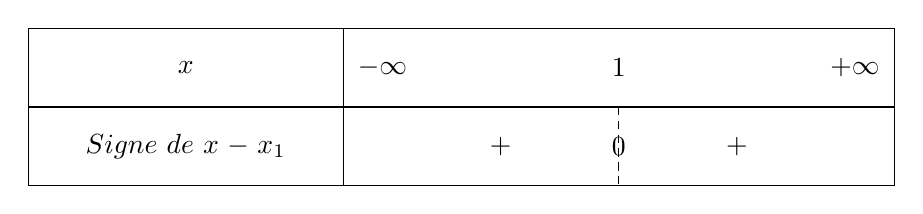
\begin{tikzpicture}
\tikzset{t style/.style = {style = densely dashed}}
\tkzTabInit[lgt=4,espcl=3]%
{$x$/1,$Signe~de~x-x_1$/1}{$-\infty$,$1$,$+\infty$}%
\tkzTabLine{, +,z,+,}
\end{tikzpicture}
\end{center}

\raggedright\\
\textbf{Pour} \mathbf{\Delta} \textbf{= 0 on a :}\\

\begin{center}
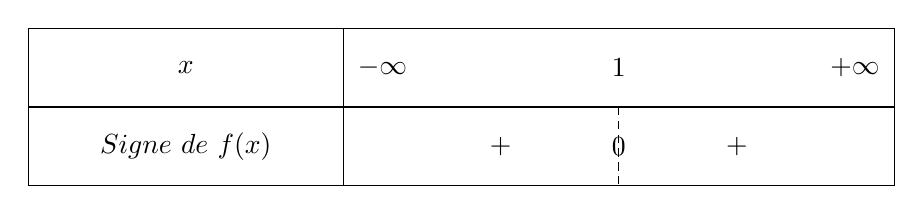
\begin{tikzpicture}
\tikzset{t style/.style = {style = densely dashed}}
\tkzTabInit[lgt=4,espcl=3]%
{$x$/1,$Signe~de~f(x)$/1}{$-\infty$,$1$,$+\infty$}%
\tkzTabLine{, +,z,+,}
\end{tikzpicture}
\end{center}

\raggedright\\
\textbf{Pour} \mathbf{\Delta} \textbf{< 0 on a :}\\

\begin{center}
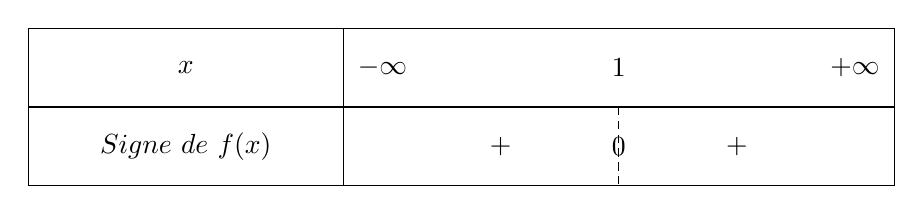
\begin{tikzpicture}
\tikzset{t style/.style = {style = densely dashed}}
\tkzTabInit[lgt=4,espcl=3]%
{$x$/1,$Signe~de~f(x)$/1}{$-\infty$,$1$,$+\infty$}%
\tkzTabLine{, +,z,+,}
\end{tikzpicture}
\end{center}

\end{document}